\section{Methods}
\subsection{Technologies Used}
For collaboration on this project we decided to use a centrally hosted IPython Jupyter Notebook server, this enabled us to use the power and availability of a provisioned server while all being able to collaborate in real time. The programming language we used was python 3 with the common data processing and machine learning packages such as sklearn, numpy and pandas.
\subsection{Dataset}
The Dataset used here is the Ames Dataset \cite{cock_2011} which is based of housing sales from between 2006 and 2010 in Ames, Iowa.
It is based on a real dataset from the municipality in Ames, but has been cleaned up to make it more suitable for the task of linear regression.
This cleanup consistent of a filtering to only include residential properties and removal of all previous sales of a property that has been sold multiple times.
Also, some of the categorical features have been modified to be more easily understandable and provide some more information. This only concerns naming and no effective change on the data though.
The dataset contains 2930 observations with 80 features, of those are roughly half categorical and half continuous. Features include many different area measurements of the house, such as basement size, living room size etc. and various counts of available facilities (such as bathrooms, kitchens, bedrooms above ground...). Categorical features include data about the location (neihgbourhood, street name etc.), the kind of heating, the style of the roof top and others.
Non of the data have been changed, the only changes have been the removal of some columns or rows. Therefore this dataset can be considered a real dataset.
\subsection{Data Preprocessing}
We are using a real dataset, that means that we first have to deal with outliers and missing data. Both the training and test dataset were treated together in the following ways:
Missing Data:\newline
Two different approaches were used to deal with missing data in our dataset. To understand what was needed, first we analysed how much data was missing on a per-feature-basis. Some features showed a high proportion of missing values, while others had fewer observations in which the value was missing.

\begin{figure}[h!]
  \centering
  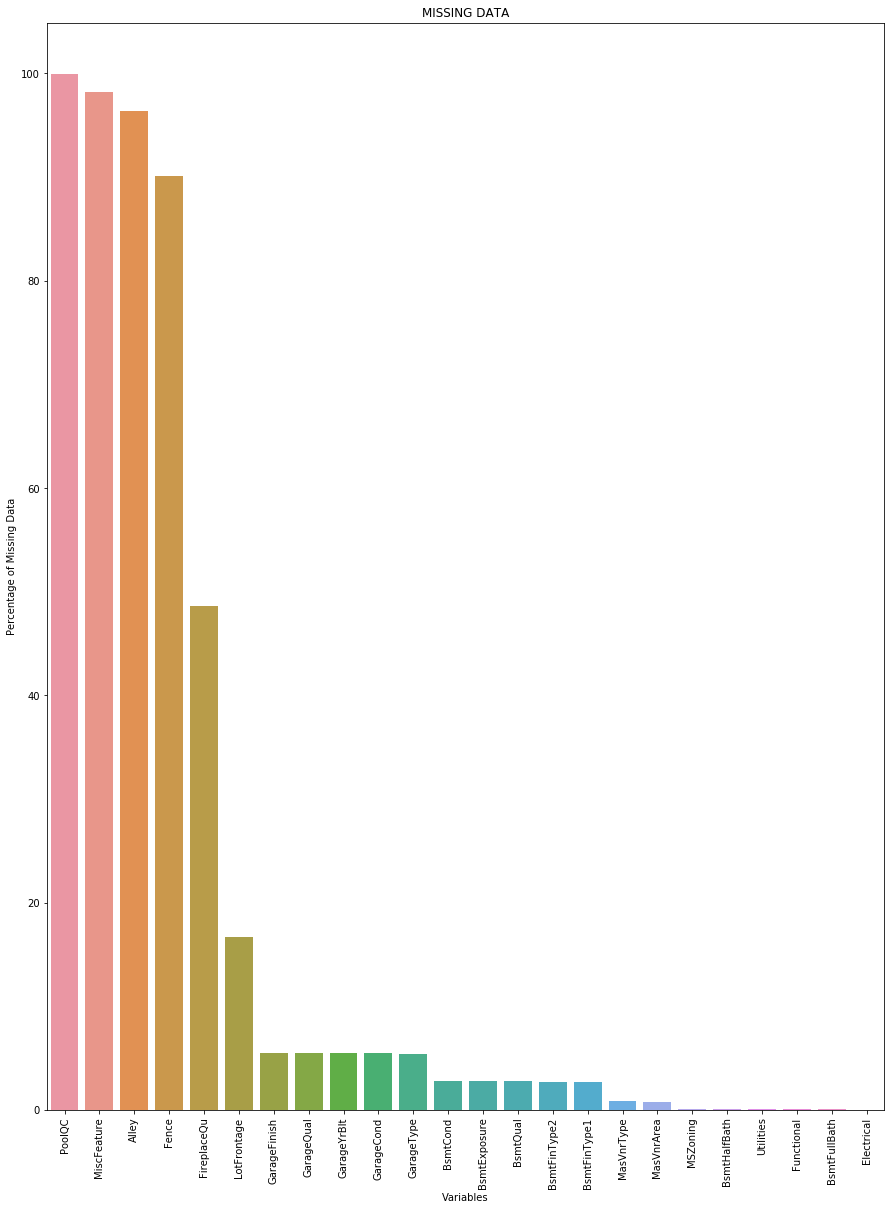
\includegraphics[width=0.4\textwidth]{images/missing-data-count-chart.png}
  \caption{Missing data per feature}
  \label{fig:missing}
\end{figure}

Features were split into two categories based on the percentage of missing data, with the split set at 50\%. Features that had more than 50\% of entries missing were removed from the dataset, while we used replacement by the mean or media for the missing entries in the remaining features.\newline
Distribution:\newline
The target value is the sales price. For linear regression with the sum of squared errors loss function, we are essentially assume the target to be normally distributed. By looking at the distribution of the price data\ref{dist-1} we can see that it is not normally distributed. To make up for this the logarithm of the price was taken, which left us with a distribution which comes very close to the normal distribution\ref{dist-2}.

\begin{figure}[h!]
  \centering
  \begin{subfigure}[b]{0.4\linewidth}
    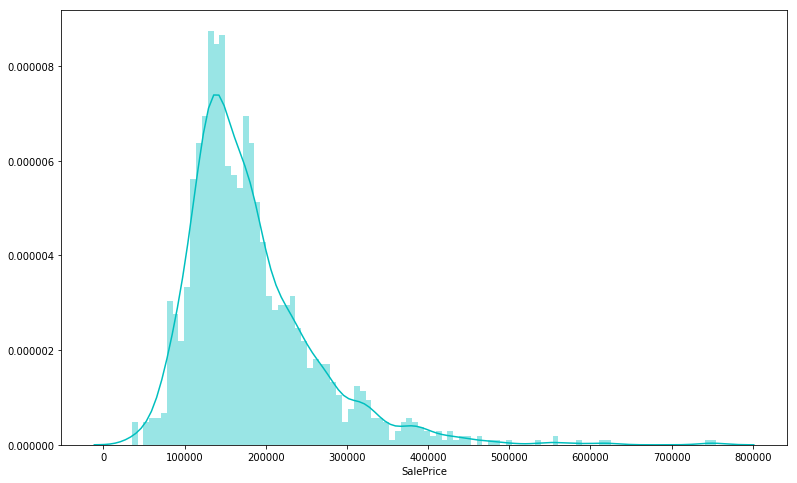
\includegraphics[width=\linewidth]{images/price_distribution.png}
    \label{fig:dist-1}
    \caption{Distribution of price}
  \end{subfigure}
  \begin{subfigure}[b]{0.4\linewidth}
    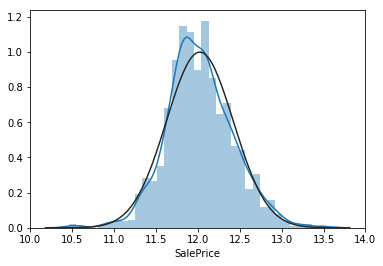
\includegraphics[width=\linewidth]{images/price_normalize_distribution.png}
    \label{fig:dist-2}
    \caption{After normalization}
  \end{subfigure}
\end{figure}

\subsection{Outliers}
Outliers are datapoints that are very different from the rest of the data. Formally defined one would usually assume a distribution (e.g. the normal distribution) on a given datarow and assume everything below and above a certain percentile an outlier.\newline
 We chose to discard outliers, because they do not provide much vlaue for the linear regression approaches that were used to analyze the data later. Thus we removed all rows which had features below the 5 percentile or above the 90 percentile.\newline
